% Instructions to change to html version:
% Comment out:
%  minipage, multicols,columnbreak, mathbf, hrule
% Replace all:% \begin{minipage}% %%\end{minipage} %%%%%\begin{mulicols}  %%%%%\end{mulicols}  %%%%\columnbreak % %%%%\begin{framed} %%%%%\endframed} %%%%%\hrule
% Search for \mathbf
% Replace \\] with \[ and \) with \(
% Enclose graphics in figure environments and add captions
% Re-tag \df environments as sections, subsections, etc.
% Command Line Code to Create html version:
%First: pdflatex -shell-escape filename.tex                                   
%Second, for each figure: inkscape "filename-figure1.pdf" -o "filename-figure1.png"
% Third: htlatex filename.tex "ht5mjlatex.cfg, charset=utf-8" " -cunihtf -utf8"


\documentclass[10pt]{article}

%\usepackage{tikz, pgf,pgfplots,wasysym,array}
%\usepackage{wasysym,array}

\usepackage{amsmath,amssymb}

\ifdefined\HCode
  \def\pgfsysdriver{pgfsys-tex4ht-updated.def}
\fi 
%\ifdefined\HCode
%  \def\pgfsysdriver{pgfsys-dvisvgm4ht.def}
%\fi 
\usepackage{tikz}
\usetikzlibrary{calc,decorations.markings,arrows}
\usepackage{pgfplots}

\pgfplotsset{compat=1.12}
\usepackage{myexternalize}
\usetikzlibrary{calc,decorations.markings,arrows}
\usepackage{framed}
\usepackage[none]{hyphenat}

\input{../../../common/1336_header_test.tex}

\begin{document}

\renewcommand{\myTitle}{MATH 2330: Multivariable Calculus}

\renewcommand{\mySubTitle}{4.5: Chain Rule } %\&\\ 11.6: Directional Derivatives \& The Gradient - Part 1}
%~\hfill Name: \underline{~~~~~~~~~~~~~~~~~~~~~~~~~~~~~~~~~~~~~~~~~~~~~~~}

\lectTitle{\vspace*{-.5in}\myTitle}{\vspace*{.1in}\mySubTitle \vspace*{-.25in}}




\section*{Section 4.5: Chain Rule}

%\begin{framed}
\subsection*{Chain Rule, Case 1:}
Let \(z=f(x,y)\) where \(x=g(t), \quad y = h(t)\). Then\\
\[\dfrac{dz}{dt} = \dfrac{\partial z}{\partial x} \dfrac{dx}{dt} + \dfrac{\partial z}{\partial y} \dfrac{dy}{dt} \hspace*{3in}\]
%\end{framed}

\begin{enumerate}[{Example} 1: ]
%\addtocounter{enumi}{1}
\item (Revisited) Consider \(f(x,y)=x^2+y^2, \quad x=3t, \quad y = e^{2t}\). Compare the result from calculating \(\dfrac{df}{dt}\) using the Chain Rule with the result that you get from first rewriting \(f\) as a function of \(t\), then taking the derivative.
\vfill


\end{enumerate}

%\begin{framed}
\subsection*{Chain Rule, Case 2:}
Let \(z=f(x,y)\) where \(x=g(s,t), \quad y = h(s,t)\). Then\\
\[\dfrac{\partial z}{\partial t} = \hspace*{4in}\] 

\[\dfrac{\partial z}{\partial s} =\hspace*{4in}\]
%\end{framed}

\begin{enumerate}[{Example} 1: ]
\addtocounter{enumi}{1}
\item Consider \(g(x,y)=x^2+xy+ y^2, \quad x=3(t+s), \quad y = e^{2st}\).
 Find \(\dfrac{\partial g}{\partial s}\) and \(\dfrac{\partial g}{\partial t}\) at \((s,t) = (1,0)\).
\vfill

\item Draw a diagram to help you write out the Chain Rule for\\ \(w=f(x,y,z)\) where \(x=g(s,t), \quad y = h(s,t), \qquad z=k(s,t)\).

\vfill

\end{enumerate}

%\pagebreak

%
%
%%\vspace*{-.5in}
%\section*{Section 11.6 -  Directional Derivatives \& The Gradient:}
%
%\hspace*{-.8in}\begin{minipage}{1.25\textwidth}
%%\begin{framed}
%
%\df{\textcolor{sblack}{Definitions \& Terminology:}}
%\begin{multicols}{2}
%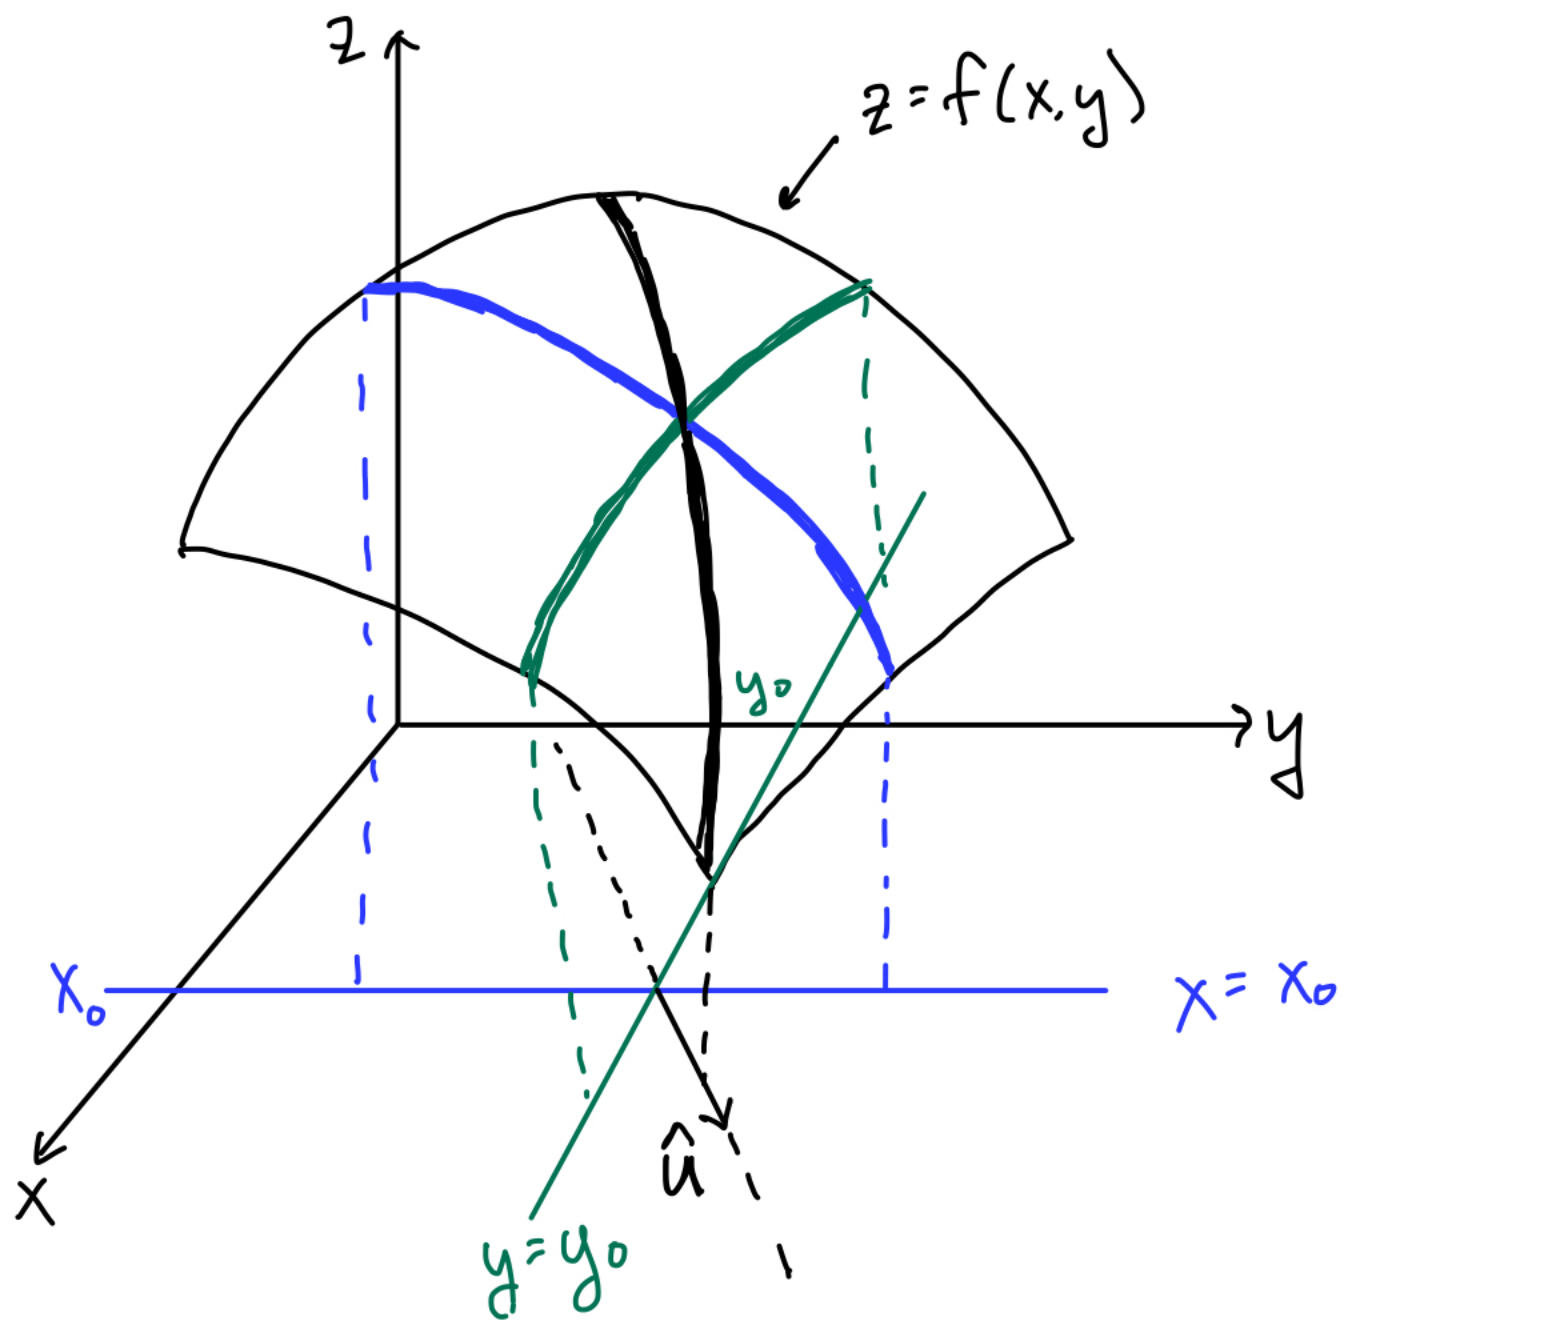
\includegraphics[width=\columnwidth]{Directional-Derivative.jpeg}
%
%
%
%\df{\textcolor{sblack}{Directional Derivative:}}~\\
%
%The \textbf{Directional Derivative} in the \(\uhat\) direction calculates the slope of the surface in the direction of the vector \(\uhat\).\\
%
% If \(f\) is a differentiable function of \(x\) and \(y\), then \(f\) has a directional derivative in the direction of any \textbf{unit vector} \(\uhat = \<a,b\>\) that can be calculated using:
%\[
%D_u f(x,y) = f_x(x,y) a + f_y(x,y) b=  \grad f \cdot \uhat\\
%\]
%
%
%\vspace*{.2in}
%
%\df{\textcolor{sblack}{The Gradient:}}
%\[
%\grad f = \<f_x,f_y\>
%\]
%
%
%\end{multicols}
%
%
%%\end{framed}
%
%\end{minipage}
%
%\textbf{Discussion:} Geometric Implications of \(D_u f(x,y) = \grad f \cdot \uhat\).
%
%\vfill

\end{document}

